\startfooter{Specialized Project: HK261-DAGD1-041\\
    Market Reconstruction
}
\part{Market Reconstruction}

Survivorship bias is a well-established problem in empirical financial research: restricting historical analysis to securities that survive until the end of the sample can produce distorted estimates and misleading evidence of return predictability. Brown et al.~\cite{Brown1992} demonstrate that survivorship-truncated samples can materially affect empirical conclusions.

\begin{figure}[H]
    \centering
    \includegraphics*[width=0.6\textwidth]{images/survivorship_bias.png}
    \caption{Survivorship Bias Illustration}
\end{figure}

For this study, avoiding survivorship bias is complicated by the limited access provided by free-tier market-data services. No single freely accessible source is assumed to provide both a sufficiently long historical security universe and the complete security-level price data required by the study. Consequently, the dataset must be reconstructed by combining complementary sources rather than directly downloaded as a finished historical panel.

\medskip

The pipeline therefore uses the \acf{NYSE} trading calendar as its temporal backbone, retrieves daily historical active-ticker snapshots from \href{https://massive.com/}{Massive \inlinelogo{images/massive-logo.png}}, aggregates these observations with Polars to derive ticker availability intervals, and uses those intervals to obtain daily \acs{OHLCV} data from Yahoo Finance. This produces a persistent raw market dataset that preserves historical security availability while remaining feasible under the constraints of the available free-tier \acs{API}s. The resulting data then serve as the foundation for the subsequent integrity checks, point-in-time universe construction, data-quality procedures, and machine-learning pipeline.

\section{Market Data Acquisition and Synthesis Pipeline}
\label{pipeline_data}
The pipeline is designed as a sequential data-reconstruction process, in which each stage produces the information required by the next rather than treating market-data acquisition as a single download operation. The central design principle is to separate historical security availability from security-level market observations. Massive's ticker-reference endpoint supports querying securities available on a specified date and filtering by active status, making it suitable for constructing the historical availability layer.

\subsection{Pipeline Architecture and Data Flow}
The first stage establishes which dates need to be processed, focusing on trading sessions actually observed on the \acs{NYSE} rather than merely using calendar days. For each trading session, Massive is queried using the date and the active-stock filter. Its \acs{API} explicitly supports retrieval of tickers available on any specified date and also returns pagination information when results exceed a single-page, allowing the complete daily snapshot to be reconstructed for each session.

\medskip

These daily snapshots are deliberately retained before aggregation, creating a two-level historical-universe representation:
\begin{enumerate}[topsep=0pt, parsep=0pt, itemsep=0pt]
    \item \textbf{Daily point-in-time snapshots}, preserving the original record of which securities were present on each trading date.
    \item \textbf{Ticker availability intervals}, providing a compact security-level summary derived from these daily observations.
\end{enumerate}

Polars transforms the first representation into the second by grouping all sessions for each ticker and taking the minimum and maximum dates:
\[
    \mathrm{start\_date}_i = \min(T_i), \qquad
    \mathrm{end\_date}_i = \max(T_i)
\]
where \(T_i\) denotes the set of observed trading dates for ticker \(i\). The resulting availability table serves as the link between universe reconstruction and downstream market-data acquisition.

\medskip

Next, Yahoo Finance is queried using these reconstructed ticker-specific intervals to download daily \acs{OHLCV} observations. Importantly, this stage does not determine historical universe membership -- that information has already been robustly reconstructed. This separation ensures that the market-data source does not implicitly define the security universe, allowing independent data integrity checks and point-in-time investment universe construction in later sections.
\begin{figure}[H]
    \centering
    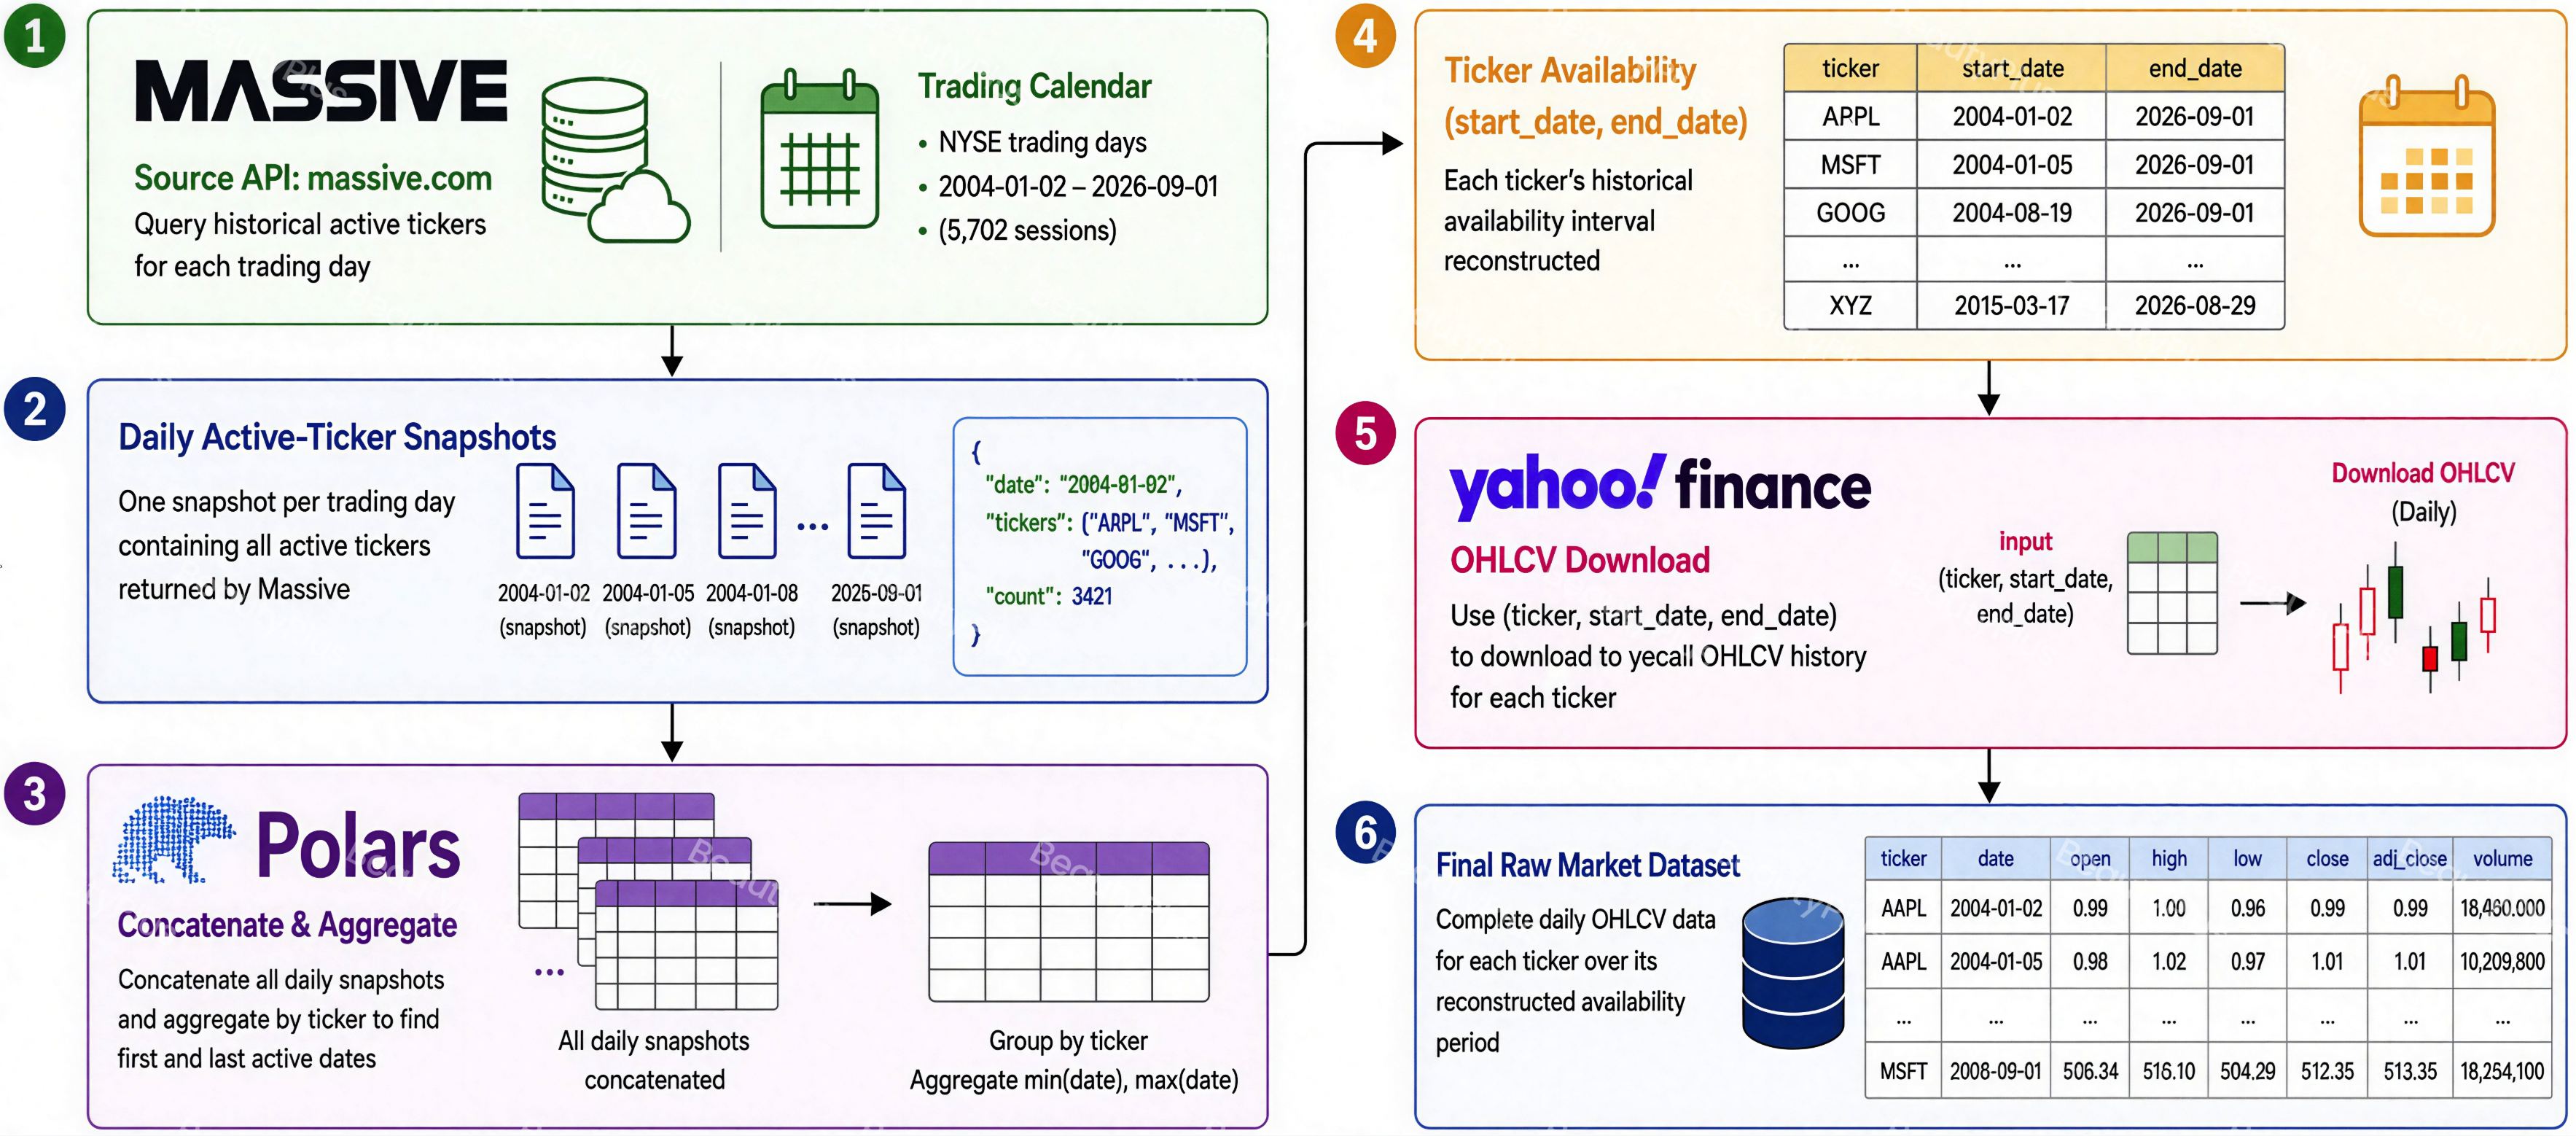
\includegraphics[width=\textwidth]{images/pipeline_data.png}
    \caption{Market Data Acquisition \& Reconstruction Pipeline}
    \label{fig:pipeline_data}
\end{figure}
Thus, the pipeline architecture can be conceptually decomposed into two connected but distinct processes:
\begin{description}
    \item[Market-data acquisition:] \hfill \\
          \textit{Ticker Availability}~$\rightarrow$~\textit{Yahoo Finance}~$\rightarrow$~\textit{Raw \acs{OHLCV} Dataset}
    \item[Historical availability reconstruction:] \hfill \\
          \textit{\acs{NYSE} Calendar}~$\rightarrow$~\textit{Massive}~$\rightarrow$~\textit{Daily Snapshots}~$\rightarrow$~\textit{Polars}~$\rightarrow$~\textit{Ticker Availability}
\end{description}

This functional separation is especially important given the constraints of free-tier data access. Instead of requiring a single source to provide a complete, survivorship-aware market panel, the pipeline distributes the reconstruction effort across complementary data providers and preserves all intermediate representations necessary for reproducibility and future audit. Notably, Massive's documentation affirms that its reference-ticker service supports historical, date-specific active-status queries -- the crucial capability leveraged in the first stages of the pipeline.

\subsection{Historical Trading Calendar and Active-Ticker Reconstruction}
The first stage establishes the \textbf{historical temporal and security universe} over which the remainder of the pipeline operates. Rather than iterating over calendar days, the pipeline first generates the official \acs{NYSE} trading sessions for the study period and then queries the historical active-ticker universe for each session. This ensures that the reconstruction is aligned with actual market activity rather than an arbitrary sequence of calendar dates. \texttt{pandas\_market\_calendars} provides exchange-specific calendars, including \acs{NYSE} holidays, regular sessions, and special market schedules.

\subsubsection*{Trading Calendar}
The study covers \textbf{2004-01-01 to 2026-09-01}. The resulting \acs{NYSE} calendar contains \textbf{5,702 trading sessions}, beginning on 2004-01-02 and ending on 2026-09-01. The calendar is generated programmatically and subsequently validated before being passed to the acquisition stage.
\begin{minted}[fontsize=\footnotesize]{python}
    def get_xnys_trading_dates(start_date: str, end_date: str) -> list[str]:
        calendar = pd_mcal.get_calendar("\acs{NYSE}")
        schedule = calendar.schedule(
            start_date=start_date,
            end_date=end_date,
        )
        return [d.strftime("%Y-%m-%d") for d in schedule.index]
\end{minted}
\begin{table}[h]
    \centering
    \small
    \begin{tabular}{l|l}
        \toprule
        \textbf{Parameter}      & \textbf{Configuration}              \\
        \hline
        Exchange                & \acs{NYSE}                          \\
        Study period            & 2004-01-01 $\rightarrow$ 2026-09-01 \\
        First trading session   & 2004-01-02                          \\
        Last trading session    & 2026-09-01                          \\
        Trading sessions        & 5,702                               \\
        Calendar implementation & \texttt{pandas\_market\_calendars}  \\
        Calendar identifier     & \texttt{\acs{NYSE}}                 \\
        \bottomrule
    \end{tabular}
    \caption{\acs{NYSE} Trading Calendar Configuration}
\end{table}
The trading-date sequence forms the pipeline's \textbf{temporal backbone}. The pipeline checks that it is non-empty, ordered, unique, and covers the target span to avoid propagating calendar errors into later \acs{API} queries.

\subsubsection*{Daily Active-Ticker Reconstruction}
For every trading session \(t\), the pipeline queries Massive's \texttt{/v3/reference/tickers} endpoint with the historical date and active-stock filters. The endpoint supports retrieving tickers available on a specified date, filtering by market and active status, with a maximum page size of 1{,}000 records and pagination through \texttt{next\_url}.
\begin{minted}[fontsize=\footnotesize]{python}
    url = "https://api.massive.com/v3/reference/tickers"
    params = {
        "date": target_date,
        "active": "true",
        "market": "stocks",
        "limit": 1000,
        "apiKey": self.api_key,
    }
\end{minted}
The resulting daily snapshot can be represented as:
\[
    S_t = \{i_1,i_2,\ldots,i_{N_t}\},
\]
where \(S_t\) denotes the set of tickers observed as active on trading session \(t\), and \(N_t\) is the corresponding number of tickers.

\medskip

The acquisition procedure for each trading session is:
\begin{enumerate}[topsep=0pt, parsep=0pt, itemsep=0pt]
    \item \textbf{Select} the next \acs{NYSE} trading session \(t\).
    \item \textbf{Query} Massive for active US stock tickers available on \(t\).
    \item \textbf{Follow pagination} until the complete response for that date has been retrieved.
    \item \textbf{Validate completion} of the entire snapshot rather than partially committing an incomplete result.
    \item \textbf{Persist} the daily ticker list as an independent raw snapshot.
    \item \textbf{Record acquisition status} in the corresponding worker manifest.
    \item \textbf{Proceed} to the next trading session.
\end{enumerate}

This design is important because each daily snapshot is treated as an independent historical observation rather than immediately collapsing the data into a single contemporary ticker list. The raw snapshots therefore preserve the temporal information required to determine when individual securities were observed as active.

\medskip

The resulting dataset has the conceptual form:
\begin{center}
    \small
    \begin{tabular}{lll}
        \toprule
        \textbf{Date} \hspace{2em} & \textbf{Active Tickers} \\
        \midrule
        2004-01-02                 & [A, AA, AACC, \dots]    \\
        2004-01-05                 & [A, AA, AACC, \dots]    \\
        2004-01-06                 & [A, AA, \dots]          \\
        \multicolumn{2}{c}{$\vdots$}                         \\
        2026-09-01                 & [A, AAPL, ABBV, \dots]  \\
        \bottomrule
    \end{tabular}
\end{center}

A further consideration is that the acquisition is subject to the practical constraints of the available \acs{API} access. Massive currently documents its Stocks Basic tier as a free tier with a \textbf{5 requests/minute} limit, making a multi-decade, date-by-date reconstruction operationally non-trivial. The pipeline therefore treats rate limiting, pagination, retries, checkpointing, and persistent storage as integral parts of the acquisition design rather than as incidental implementation details. These mechanisms are discussed together with the distributed execution strategy in the following section.

\subsection{Distributed Acquisition and Persistent Storage}

The historical reconstruction requires 5,702 trading-session queries, with each date potentially requiring multiple paginated \acs{API} requests. Under the available free-tier rate constraints, processing the entire period sequentially would make the acquisition unnecessarily slow and vulnerable to interruption. The pipeline therefore distributes the workload across independent workers while maintaining persistent checkpoints so that completed dates do not need to be downloaded again.

\subsubsection*{Distributed Execution}
\begin{figure}[H]
    \centering
    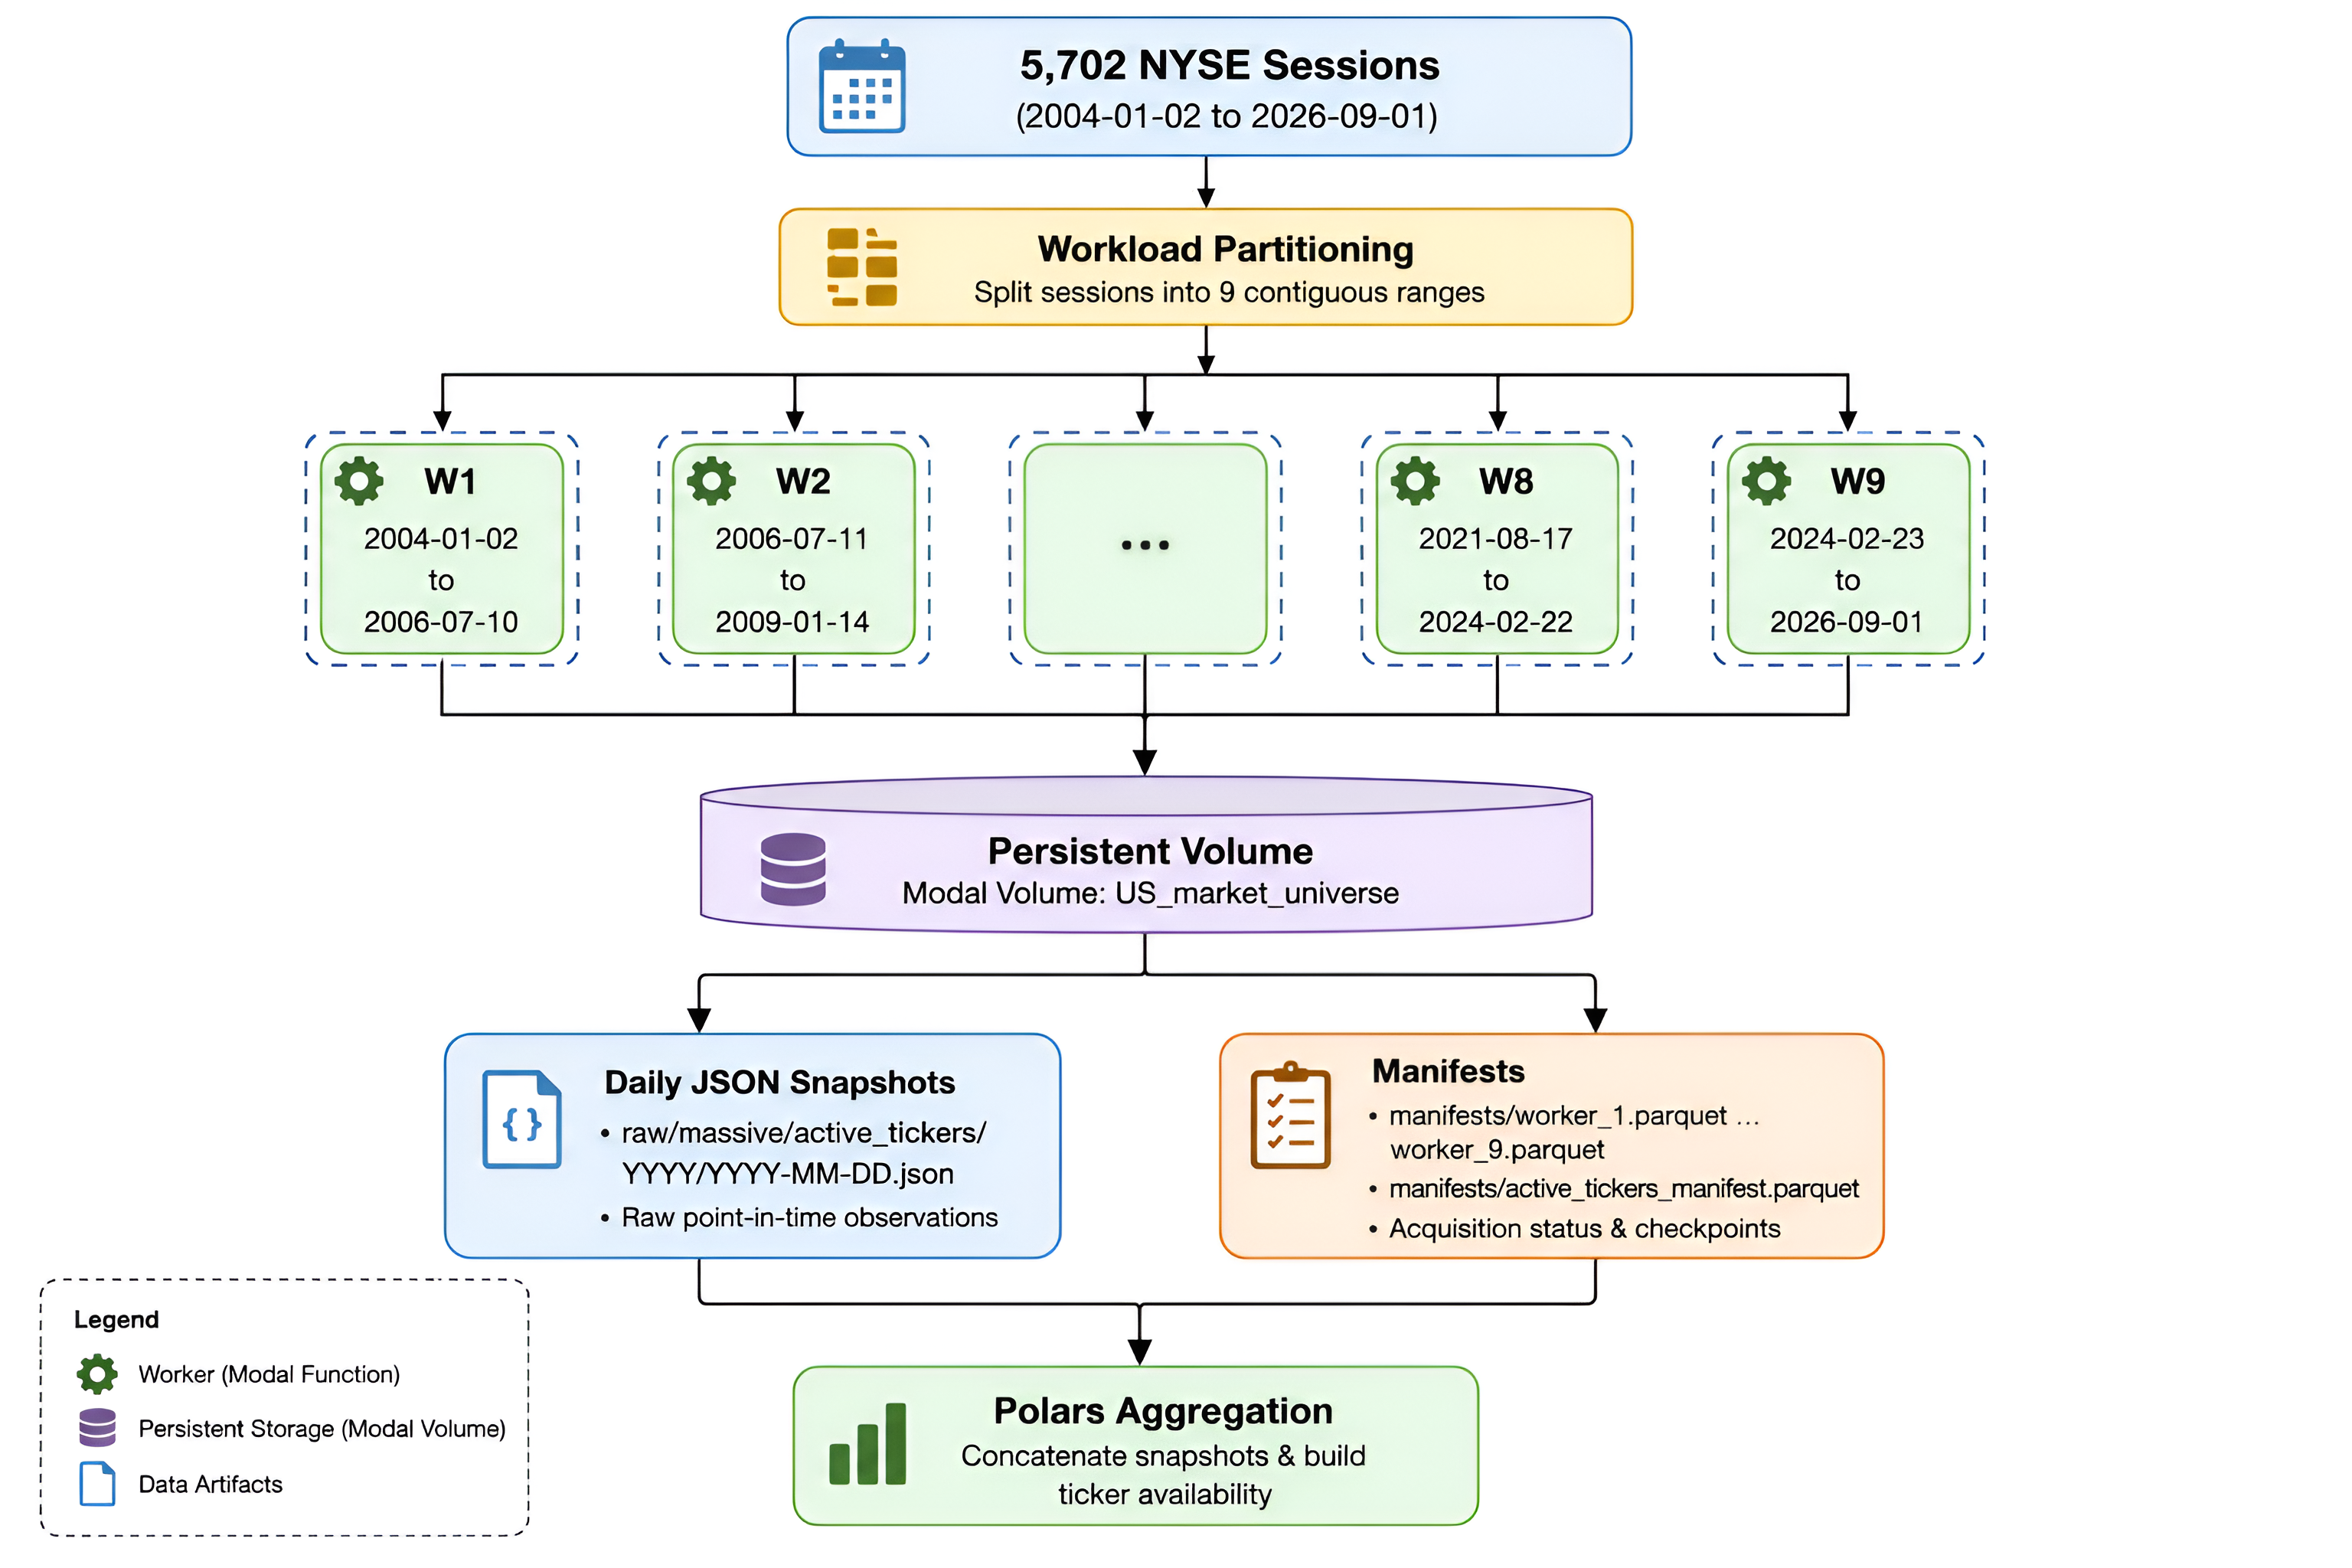
\includegraphics[width=\textwidth]{images/workers.png}
    \caption{Workers Distributed Architecture}
    \label{flow:workers}
\end{figure}

The implementation uses Modal to execute the acquisition in parallel. Modal supports remote function execution, configurable retries, secret injection, and persistent Volume storage shared across function instances.

\medskip

The 5,702 \acs{NYSE} sessions are initially divided into nine approximately equal chronological partitions, with each worker responsible for a contiguous date range. Contiguous partitioning simplifies progress tracking and makes the resulting manifests directly interpretable.

\begin{table}[H]
    \centering
    \small
    \begin{tabular}{ccl}
        \toprule
        \textbf{Worker} & \textbf{Sessions} & \textbf{Initial date range}         \\
        \midrule
        No. 1           & 634               & 2004-01-02 $\rightarrow$ 2006-07-10 \\
        No. 2           & 634               & 2006-07-11 $\rightarrow$ 2009-01-14 \\
        No. 3           & 634               & 2009-01-15 $\rightarrow$ 2011-07-21 \\
        No. 4           & 634               & 2011-07-22 $\rightarrow$ 2014-01-29 \\
        No. 5           & 634               & 2014-01-30 $\rightarrow$ 2016-08-04 \\
        No. 6           & 633               & 2016-08-05 $\rightarrow$ 2019-02-11 \\
        No. 7           & 633               & 2019-02-12 $\rightarrow$ 2021-08-16 \\
        No. 8           & 633               & 2021-08-17 $\rightarrow$ 2024-02-22 \\
        No. 9           & 633               & 2024-02-23 $\rightarrow$ 2026-09-01 \\
        \midrule
        \textbf{Total}  & 5,702             & 2004-01-02 $\rightarrow$ 2026-09-01 \\
        \bottomrule
    \end{tabular}
    \caption{Parallel \acs{NYSE} Worker Splits.}
    \label{tab:parallel-nyse-worker-splits}
\end{table}

Each worker operates independently and uses a dedicated Massive \acs{API} credential. This isolates rate-limit consumption between workers while allowing the nine partitions to progress concurrently. The workers are spawned simultaneously, after which their execution results are collected by the orchestration process.

\medskip

The distributed design also incorporates checkpoint-aware workload redistribution. Before assigning work, the orchestration layer examines the persistent manifests to identify dates that have already been completed. Consequently, if a worker terminates after successfully processing part of its assigned interval, subsequent execution does \emph{not} restart the entire interval. Remaining dates can instead be redistributed among available workers. This is particularly important for a long-running acquisition where transient \acs{API} failures or worker interruptions should not invalidate previously completed work.

\subsubsection*{Rate Limiting and Fault Tolerance}
Because the acquisition is constrained by \acs{API} request limits, each worker explicitly controls its request rate. The implementation uses a fixed inter-page delay and exponential-style backoff for transient failures.

\begin{center}
    \small
    \begin{tabular}{ll}
        \toprule
        \textbf{Mechanism}     & \textbf{Configuration}             \\
        \midrule
        Inter-page delay       & 12 seconds                         \\
        Initial retry backoff  & 3 seconds                          \\
        Maximum retry backoff  & 30 seconds                         \\
        Maximum retries        & 10                                 \\
        Completion requirement & Entire daily snapshot must succeed \\
        Checkpoint unit        & Individual trading session         \\
        \bottomrule
    \end{tabular}
\end{center}

A daily snapshot is not committed as successful merely because the first \acs{API} response was received. The worker continues through \emph{all} pagination and only records the date as successfully completed after the complete ticker set has been retrieved. This prevents partially retrieved pages from being interpreted as a valid historical universe.

\medskip

This distinction is important because an incomplete snapshot would not necessarily generate an obvious runtime error; it could instead silently produce an artificially small historical universe. The acquisition process therefore treats completeness of each date-level snapshot as a prerequisite for persistence.

\subsubsection*{Persistent Storage and Checkpointing}
All workers access a shared Modal Volume named \texttt{US\_market\_universe}. Modal Volumes provide persistent filesystem-like storage that can be shared by multiple functions and retained across separate executions. Changes must be committed to make them durably available to other containers.

    {\small
        \dirtree{%
            .1 /mnt/data/.
            .2 raw/.
            .3 massive/.
            .4 active\_tickers/.
            .5 2004/.
            .6 2004-01-02.json.
            .6 2004-01-05.json.
            .6 \dots.
            .5 2005/.
            .5 \dots.
            .2 manifests/.
            .3 worker\_1.parquet.
            .3 worker\_2.parquet.
            .3 \dots.
            .3 worker\_9.parquet.
            .3 active\_tickers\_manifest.parquet.
        }
    }

The separation between raw snapshots and manifests serves two different purposes:
\begin{center}
    \small
    \begin{tabular}{p{0.28\linewidth} p{0.67\linewidth}}
        \toprule
        \textbf{Artifact}     & \textbf{Purpose}                                                \\
        \midrule
        Daily JSON snapshot   & Preserve the actual historical ticker observation               \\
        Worker manifest       & Record which dates succeeded or failed                          \\
        Consolidated manifest & Provide a global acquisition-status record                      \\
        Modal Volume          & Provide persistent shared storage across workers and executions \\
        \bottomrule
    \end{tabular}
\end{center}

The manifests therefore function as the pipeline's checkpoint layer. On a subsequent execution, the system reads the manifests and identifies already completed dates before assigning remaining work. This makes the acquisition resumable and prevents successful \acs{API} requests from being unnecessarily repeated.

\medskip

Each raw daily snapshot follows a compact structure:
\begin{minted}[fontsize=\footnotesize]{json}
    {
    "date": "YYYY-MM-DD",
    "tickers": ["AAPL", "MSFT", "NVDA", "..."],
    "ticker_count": 3667
    }
\end{minted}
The result is a fault-tolerant acquisition layer rather than a one-shot scraping process. Raw observations remain available independently of worker execution state, while manifests provide sufficient information to resume incomplete portions of the historical period. This persistent intermediate layer is subsequently consumed by the ticker-availability reconstruction described in Section~\ref{sec:ticker_availability}. Modal's documentation also notes that concurrent modification of the same Volume files should be avoided; accordingly, the implementation assigns separate snapshot files to dates and separate manifest files to workers rather than having multiple workers overwrite the same file.

\subsection{Ticker Availability Reconstruction}
\label{sec:ticker_availability}

\subsection{Security-Level \acs{OHLCV} Acquisition}
\label{sec:yahoo_ingestor}



\clearpage
\section{Data Integrity}
\subsection{Data Quality and Missing Observations}

\section{Factor Data}

To facilitate the systematic risk residualization required for the cross-sectional prediction target, external macroeconomic factor data must be integrated into the pipeline. The daily Fama-French 3-Factor dataset\cite{FamaFrench1992} is acquired programmatically via \texttt{pandas-datareader} directly from the Kenneth R. French Data Library. This dataset provides the daily market risk premium ($\mathrm{Mkt\text{-}RF}$), the size factor ($\mathrm{SMB}$), the value factor ($\mathrm{HML}$), and the risk-free rate ($\mathrm{RF}$).

\medskip

A critical MLOps engineering consideration in acquiring this factor data is chronological alignment and the management of publication lag. Because the Kenneth R. French Data Library operates with an inherent reporting delay relative to live equity markets, the overall observation period of the analytical sample is dynamically truncated to match the maximum available factor date. This strict date intersection prevents the introduction of missing observations into the trailing 126-day rolling OLS regressions and explicitly prohibits the use of forward-filling techniques, which would otherwise introduce forward-looking data leakage into the residualized alpha target.

\section{Point-in-Time Universe Construction}